\chapter{Graph Coloring}
\lecture{18}{12 May.}{}
\begin{eg}[Motivation Example: Course scheduling]
    The department offers \(n\) courses, and they want to schedule them so that there are no two courses that any student is interested in occuring at the same time. At the same time, we aim to use as few time as possible.   
\end{eg}

We can build a conflict graph, where vertices for courses and edges for pairs of courses that shouldn't clash. Need to assign a time slot to each course, such that adjacent vertices receive different time slots, and at the same time we aim to minimize the number of slots we use.

\begin{definition}
    Given a graph \(G = (V, E)\), a \(k\)(-vertex) coloring of \(G\) is an assignment of use of \(k\) colors to each vertex, i.e. \(\varphi : V \to [k]\). The coloring is \emph{proper} if \(\varphi (u) \neq \varphi (v)\) for all \(\left\{ u, v \right\} \in E \). The \emph{chromatic number} of \(G\) is the smallest \(k\) for which a proper \(k\)-coloring exists, denote \(\chi (G)\).          
\end{definition}

\begin{eg}
    \(\chi (K_n) = n\). 
\end{eg}

\begin{remark}
    If \(G\) has \(n\) vertices, then \(\chi (G) \le n\).   
\end{remark}

\begin{remark}
    If \(H \subseteq G\), then \(\chi (H) \le \chi (G)\). Hence, if \(G\) has a clique of order \(k\), then \(\chi (G) \ge \chi (K_k) = k\).      
\end{remark}

\begin{claim}
    \(\chi (G) \ge \omega (G) \coloneqq \max \left\{ k \mid K_k \subseteq G \right\} \). 
\end{claim}

\begin{definition}
    \(G\) is bipartite iff \(\chi (G) \le 2\).  
\end{definition}

\begin{remark}
    This definition is equivalent to the one we learnt before. If \(\chi (G) = 2\), we can just separate the vertices with color 1 to one side and the other vertices with color 2 to the other side, and thus \(G\) is bipartite. 
\end{remark}

\paragraph{Decision problems:}
\begin{itemize}
    \item Is \(\chi (G) \le 2\)? is in \(P\). 
    \item Is \(\chi (G) \le k\) for any \(k \ge 3\)? is NP-complete.    
\end{itemize}

\begin{question}
    How can we show that \(\chi (G) > k\)? i.e. what lower bound can we give on \(\chi (G)\)?  
\end{question}

We have shown that \(\chi (G) \ge \omega (G)\). Now we can give another lower bound:
\begin{theorem}[Mycielski]
    For any \(k \in \mathbb{N}\), there is a triangle-free graph \(G_k\) with \(\chi (G_k) \ge k\).   
\end{theorem} 

\begin{proof}
    For \(k = 1\), \(G_1\) can be the singleton, where if \(k = 2\), \(G_2\) can be \((\left\{ u, v \right\}, \left\{ (u, v) \right\} )\), while for \(k = 3\), \(G_3\) can be \(C_5\).

    \textbf{Mycielski's construction:} Given \(G_k\), construct \(G_{k+1} \). Let \(V(G_k) = \left\{ v_1, v_2, \dots , v_n \right\} \). We can introduce new vertices \(u_1, u_2, \dots , u_n\) and \(w\), where the edges of \(G_{k+1}\) are:
    for every \(\left\{ v_i, v_j \right\} \in E(G_k) \), add edges \(\left\{ v_i, v_j \right\}, \left\{ u_i, v_j \right\}, \left\{ v_i, u_j \right\}   \) to \(E(G_{k+1})\). Finally, we add \(\left\{ u_i, w \right\} \) to \(E(G_{k+1})\) for all \(i\). 
    \begin{figure}[H]
        \centering
        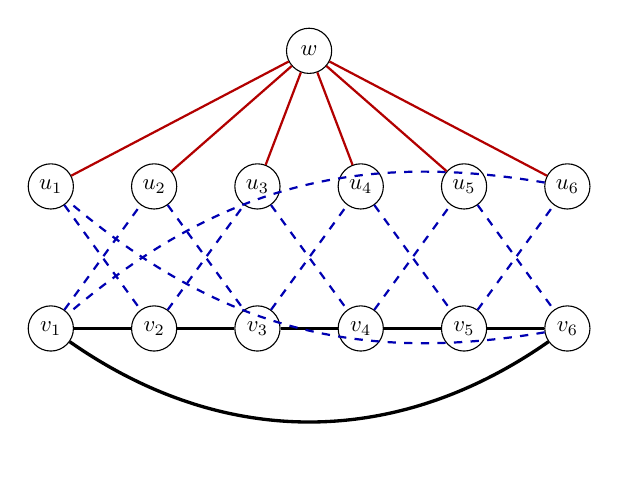
\begin{tikzpicture}[
            scale=0.82,
            every node/.style={transform shape},
            vertex/.style={circle, draw, fill=white, minimum size=7mm, inner sep=0pt},
            original/.style={very thick},
            crossedge/.style={blue!70!black, thick, dashed},
            apexedge/.style={red!70!black, thick}
        ]
            \foreach \i/\x in {1/0,2/1.6,3/3.2,4/4.8,5/6.4,6/8.0} {
                \node[vertex] (v\i) at (\x,0) {$v_\i$};
                \node[vertex] (u\i) at (\x,2.2) {$u_\i$};
            }
            \node[vertex] (w) at (4,4.3) {$w$};

            \draw[original] (v1) -- (v2);
            \draw[original] (v2) -- (v3);
            \draw[original] (v3) -- (v4);
            \draw[original] (v4) -- (v5);
            \draw[original] (v5) -- (v6);
            \draw[original, bend left=35] (v6) to (v1);

            \draw[crossedge] (u1) -- (v2);
            \draw[crossedge] (v1) -- (u2);
            \draw[crossedge] (u2) -- (v3);
            \draw[crossedge] (v2) -- (u3);
            \draw[crossedge] (u3) -- (v4);
            \draw[crossedge] (v3) -- (u4);
            \draw[crossedge] (u4) -- (v5);
            \draw[crossedge] (v4) -- (u5);
            \draw[crossedge] (u5) -- (v6);
            \draw[crossedge] (v5) -- (u6);
            \draw[crossedge, bend right=25] (u6) to (v1);
            \draw[crossedge, bend left=25] (v6) to (u1);

            \foreach \i in {1,...,6} {
                \draw[apexedge] (w) -- (u\i);
            }

        \end{tikzpicture}
    \end{figure}
    \begin{claim}
        \(G_{k+1}\) is triangle-free. 
    \end{claim}                  
    \begin{explanation}
        Since \(G_k\) is triangle free, any triangle includes a new vertex. Since \(w\) is only adjacent to the \(u_i\)'s, and the \(u_i\)'s are independent, triangle must be of the form 
        \[
            u_i, v_j, v_{\ell }, \quad i \neq j, \ell , \quad j \neq \ell.
        \]    
        If there is a triangle, then so is \(v_i, v_j, v_{\ell} \subseteq G_k\), which is a contradiction.
    \end{explanation}

    \begin{claim}
        \(\chi (G_{k+1}) = k + 1\). 
    \end{claim}
    \begin{explanation}
        \hfill 
        \begin{itemize}
            \item [(\(\le\))] Given a \(k\)-coloring \(\varphi _k\) of \(G_k\), define 
            \[
                \varphi _{k+1}(x) = \begin{dcases}
                    \varphi _k(v_i), &\text{ if } x \in \left\{ v_{i} \text{'s} , u_i \text{'s}  \right\}  ;\\
                    k + 1, &\text{ if } x = w.
                \end{dcases}
            \]
            \item [(\(\ge\))] Suppose \(\varphi \) is a (proper) \(k\)-coloring of \(G_{k+1}\). WLOG, \(\varphi (w) = k\), then \(\varphi (\left\{ u_1, \dots , u_n \right\} ) \subseteq [k - 1]\). Define \(\psi : V(G_k) \to [k - 1]\), where 
            \[
                \psi (v_i) = \begin{dcases}
                    \varphi (v_i), &\text{ if } \varphi (v_i) \neq k ;\\
                    \varphi (u_i), &\text{ if } \varphi (v_i) = k .
                \end{dcases}
            \]
            This gives a proper \(k - 1\)-coloring of \(G_k\), which contradicts to \(\chi (G_k) \ge k\).  
        \end{itemize}
    \end{explanation}
\end{proof}

\begin{observation}
    In any proper coloring, each color class \(\left\{ v: \varphi (v) = i \right\} \) is an independent set.  
\end{observation}

Recall that 
\[
    \alpha (G) = \max \left\{ \vert S \vert: S \subseteq V \text{ is independent}   \right\}, 
\]
then we have the claim 
\begin{claim}
    \(\chi (G) \ge \frac{n}{\alpha (G)}\), where \(n = \vert V(G) \vert \).
\end{claim}
\begin{explanation}
    \[
        n = \sum_{k=1}^{\chi(G)} \vert S_k \vert \le \sum_{k=1}^{\chi(G)} \alpha (G) = \alpha (G) \cdot \chi(G),   
    \]
    where \(S_k\) is the independent set formed by the vertices of color \(k\).  
\end{explanation}

\begin{remark}
    Suppose \(G \sim G \left( n, \frac{1}{2} \right) \), i.e. uniformly random (labelled) graph on \(n\) vertices, then 
    \[
        \alpha (G) \thickapprox 2 \log _2 n, \quad \omega (G) \thickapprox 2\log _2 n,
    \]  
    and we have 
    \[
        \chi (G) \gtrsim \frac{n}{2 \log _2 n},
    \]
    which is asymptotically tight.
\end{remark}

\paragraph{Upper bounds on \(\chi (G)\)}

\begin{claim}
    \(\chi (G) \le \Delta (G) + 1\).  
\end{claim}

\begin{explanation}
    We can use a greedy strategy: Order vertices \(v_1, \dots , v_n\), then consider the vertices one at a time. When considering \(v_i\), give it the smallest color that doesn't appear in the earlier neighbors. Since \(v_i\) has at most \(\Delta (G)\) earlier neighbors, we always have an available color in \(\left\{ 1, 2, \dots , \Delta (G) + 1 \right\} \). Thus, we get a proper coloring with \(\le \Delta (G) + 1\) colors.      
\end{explanation}

\paragraph{Bound in best possible}
\begin{eg}
    \hfill 
    \begin{itemize}
        \item \(G = K_n\), then \(\chi (G) = n\) and \(\Delta(G) = n - 1\).
        \item \(G = C_n\), \(n\) odd, then \(\chi (G) = 3\) and \(\Delta (G) = 2\).    
    \end{itemize}   
\end{eg}

\begin{definition}
    A graph \(G\) is \(r\)-degenerate if in any subset \(S \subseteq V\), there is a vertex in \(G[S]\) of degree \(\le r\), i.e. every subgraph \(H\) of \(G\) has \(\delta (H) \le r\).       
\end{definition}

\begin{observation}
    \(\delta (G) \le r \le \Delta (G)\). 
\end{observation}

\begin{remark}
    \(G\) is \(r\)-degenerate iff there is a vertex ordering \(v_1, \dots , v_n\) s.t. each \(v_i\) has \(\le r\) neighbors before it.     
\end{remark}

\begin{proposition}
    If \(G\) is \(r\)-degenerate, then \(\chi (G) \le r + 1\).   
\end{proposition}
\begin{proof}
    Run the greedy algorithm with the degenerating order. 
\end{proof}

\begin{theorem}[Brooks' theorem]
    If \(G\) is a connected graph and \(G \neq K_n\) or (\(C_n\) for odd \(n\)), then \(\chi (G) \le \Delta (G)\).     
\end{theorem}